\section{Installing and getting familiar with BrainVISA}

BrainVISA can be downloaded from the dedicated website at \url{http://www.brainvisa.info}. Installation instructions come with the downloaded file, and are also available in the BrainVISA handbook at \url{http://brainvisa.info/doc/axon/bv_man/en/html/}. We urge users to read this handbook to get familiar with the BrainVISA environment before going further with {\em Vobi One}.

Note that the tests and validation of {\em Vobi One} were performed under a 64 bit linux operating system using BrainVISA V4.3.0. Therefore, using the same version of BrainVISA is mandatory. We also recommend a 64 bit linux operating system to use {\em Vobi One}, even if there is a high chance that everything should work fine with others.

To install BrainVISA, simply download the archive into the directory of your choice and unpack it.

\begin{verbatim}
    > cd /mydirectory
    > tar xvfj brainvisa-Mandriva-2008.0-x86_64-4.3.0-2012_09_03.tar.bz2
\end{verbatim}

We recommend that you choose \texttt{/mydirectory} to have the full permissions to read and write what you need (for instance, it can be your home directory \texttt{/home/login}). In particular, we recommend not to install BrainVISA system-wide as root, which will ease some further steps. Once you have executed this \texttt{tar} command, the file \texttt{brainvisa-Mandriva-2008.0-x86\_64-4.3.0-2012\_09\_03.tar.bz2} is no longer needed; you can remove it, unless you want to reinstall BrainVISA.

A directory called \texttt{brainvisa-4.3.0} will be created. We will refer to \texttt{/mydirectory/brainvisa-4.3.0} as the BrainVISA installation directory. You will find installation instructions and other useful information in a \texttt{README} file in that directory. To launch BrainVISA, simply run the corresponding executable by typing its full path. Add the \& sign at the end to keep an active shell prompt (optional).

\begin{verbatim}
    > /mydirectory/brainvisa-4.3.0/bin/brainvisa &
\end{verbatim}

\section{Installing {\em Vobi One}}

{\em Vobi One} can be downloaded from the dedicated website at \url{https://trac.int.univ-amu.fr/vobi_one}. Once you have downloaded the toolbox file into \texttt{/mydirectory}, the first thing to do is to unpack the downloaded archive:

\begin{verbatim}
    > cd /mydirectory
    > tar xvfz vobi_one_vX.XX_cYYY.tgz
\end{verbatim}

This will create a directory called \texttt{vobi\_one\_src}. To install {\em Vobi One}, you simply need to go to this directory, and then copy some content inside the BrainVISA installation directory.

\begin{verbatim}
    > cd /mydirectory/vobi_one_src
    > cp -rf lib/ brainvisa/ /mydirectory/brainvisa-4.3.0
\end{verbatim}


To check that the installation was successfull, you should restart BrainVISA. You will be asked to update a database, and you should proceed. Then make sure that the {\em Vobi One} icon now appears in the toolbox panel on the left side of the main BrainVISA interface, as illustrated on Fig.~\ref{fig:bv_gui_v1_install}.

\begin{figure}[!h]
\begin{center}
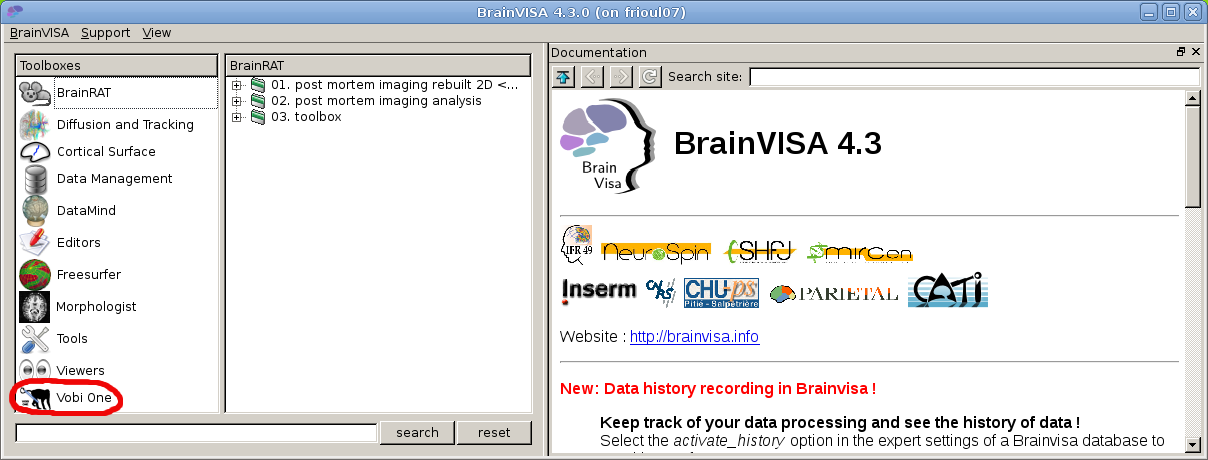
\includegraphics[width=12cm]{figs/brainvisa_gui_v1_install.png}
\caption{If the installation of {\em Vobi One} is successfull, you should see the icon circled in red.}
\label{fig:bv_gui_v1_install}
\end{center}
\end{figure}

Finally, you need to update the documentation of BrainVISA to include the {\em Vobi One} documentation. This process, which will take several minutes, can be launched by typing the following command:

\begin{verbatim}
    > /mydirectory/brainvisa-4.3.0/bin/brainvisa --noMainWindow --updateDocumentation
\end{verbatim}

Once you have done all this successfully, you can clean up some files and directory that are not needed anymore (unless you want to reinstall {\em Vobi One}):

\begin{verbatim}
    > rm -rf /mydirectory/vobi_one_src
    > rm /mydirectory/vobi_one_vX.XX_cYYY.tgz
\end{verbatim}



\section{Setting up BrainVISA to use Vobi One}
Before being able to use {\em Vobi One}, you need to define a BrainVISA database. We recommend reading the documentation of the {\em Data Management} toolbox available in the BrainVISA interface to learn more about BrainVISA databases.

In order to create a database, the first time you launch BrainVISA, go to the following menu item: 
BrainVISA - Preferences - Databases - Add...,  and select (or create) the root directory for your database (let's call it \texttt{/brainvisadatabase}).
Make sure this directory is located on a ressource where enough space is available to store all the raw data, the intermediary
files and the results of your future analyses.

You are now ready to go!

\section{Preparing the demo dataset}

A demonstration dataset is available at \url{https://trac.int.univ-amu.fr/vobi_one}. Once you have downloaded it, unpack the archive in the directory of your choice. We strongly recommend that this should not be in the root directory you defined for your BrainVISA database.

\begin{verbatim}
    > cd /rawdatadirectory
    > tar xvfj vobi_one_demo_data.tar.bz2
\end{verbatim}
